% Options for packages loaded elsewhere
\PassOptionsToPackage{unicode}{hyperref}
\PassOptionsToPackage{hyphens}{url}
%
\documentclass[
]{article}
\title{Math Stat Final Project -- Deriving Estimators}
\author{}
\date{\vspace{-2.5em}}

\usepackage{amsmath,amssymb}
\usepackage{lmodern}
\usepackage{iftex}
\ifPDFTeX
  \usepackage[T1]{fontenc}
  \usepackage[utf8]{inputenc}
  \usepackage{textcomp} % provide euro and other symbols
\else % if luatex or xetex
  \usepackage{unicode-math}
  \defaultfontfeatures{Scale=MatchLowercase}
  \defaultfontfeatures[\rmfamily]{Ligatures=TeX,Scale=1}
\fi
% Use upquote if available, for straight quotes in verbatim environments
\IfFileExists{upquote.sty}{\usepackage{upquote}}{}
\IfFileExists{microtype.sty}{% use microtype if available
  \usepackage[]{microtype}
  \UseMicrotypeSet[protrusion]{basicmath} % disable protrusion for tt fonts
}{}
\makeatletter
\@ifundefined{KOMAClassName}{% if non-KOMA class
  \IfFileExists{parskip.sty}{%
    \usepackage{parskip}
  }{% else
    \setlength{\parindent}{0pt}
    \setlength{\parskip}{6pt plus 2pt minus 1pt}}
}{% if KOMA class
  \KOMAoptions{parskip=half}}
\makeatother
\usepackage{xcolor}
\IfFileExists{xurl.sty}{\usepackage{xurl}}{} % add URL line breaks if available
\IfFileExists{bookmark.sty}{\usepackage{bookmark}}{\usepackage{hyperref}}
\hypersetup{
  pdftitle={Math Stat Final Project -- Deriving Estimators},
  hidelinks,
  pdfcreator={LaTeX via pandoc}}
\urlstyle{same} % disable monospaced font for URLs
\usepackage[margin=1in]{geometry}
\usepackage{color}
\usepackage{fancyvrb}
\newcommand{\VerbBar}{|}
\newcommand{\VERB}{\Verb[commandchars=\\\{\}]}
\DefineVerbatimEnvironment{Highlighting}{Verbatim}{commandchars=\\\{\}}
% Add ',fontsize=\small' for more characters per line
\usepackage{framed}
\definecolor{shadecolor}{RGB}{248,248,248}
\newenvironment{Shaded}{\begin{snugshade}}{\end{snugshade}}
\newcommand{\AlertTok}[1]{\textcolor[rgb]{0.94,0.16,0.16}{#1}}
\newcommand{\AnnotationTok}[1]{\textcolor[rgb]{0.56,0.35,0.01}{\textbf{\textit{#1}}}}
\newcommand{\AttributeTok}[1]{\textcolor[rgb]{0.77,0.63,0.00}{#1}}
\newcommand{\BaseNTok}[1]{\textcolor[rgb]{0.00,0.00,0.81}{#1}}
\newcommand{\BuiltInTok}[1]{#1}
\newcommand{\CharTok}[1]{\textcolor[rgb]{0.31,0.60,0.02}{#1}}
\newcommand{\CommentTok}[1]{\textcolor[rgb]{0.56,0.35,0.01}{\textit{#1}}}
\newcommand{\CommentVarTok}[1]{\textcolor[rgb]{0.56,0.35,0.01}{\textbf{\textit{#1}}}}
\newcommand{\ConstantTok}[1]{\textcolor[rgb]{0.00,0.00,0.00}{#1}}
\newcommand{\ControlFlowTok}[1]{\textcolor[rgb]{0.13,0.29,0.53}{\textbf{#1}}}
\newcommand{\DataTypeTok}[1]{\textcolor[rgb]{0.13,0.29,0.53}{#1}}
\newcommand{\DecValTok}[1]{\textcolor[rgb]{0.00,0.00,0.81}{#1}}
\newcommand{\DocumentationTok}[1]{\textcolor[rgb]{0.56,0.35,0.01}{\textbf{\textit{#1}}}}
\newcommand{\ErrorTok}[1]{\textcolor[rgb]{0.64,0.00,0.00}{\textbf{#1}}}
\newcommand{\ExtensionTok}[1]{#1}
\newcommand{\FloatTok}[1]{\textcolor[rgb]{0.00,0.00,0.81}{#1}}
\newcommand{\FunctionTok}[1]{\textcolor[rgb]{0.00,0.00,0.00}{#1}}
\newcommand{\ImportTok}[1]{#1}
\newcommand{\InformationTok}[1]{\textcolor[rgb]{0.56,0.35,0.01}{\textbf{\textit{#1}}}}
\newcommand{\KeywordTok}[1]{\textcolor[rgb]{0.13,0.29,0.53}{\textbf{#1}}}
\newcommand{\NormalTok}[1]{#1}
\newcommand{\OperatorTok}[1]{\textcolor[rgb]{0.81,0.36,0.00}{\textbf{#1}}}
\newcommand{\OtherTok}[1]{\textcolor[rgb]{0.56,0.35,0.01}{#1}}
\newcommand{\PreprocessorTok}[1]{\textcolor[rgb]{0.56,0.35,0.01}{\textit{#1}}}
\newcommand{\RegionMarkerTok}[1]{#1}
\newcommand{\SpecialCharTok}[1]{\textcolor[rgb]{0.00,0.00,0.00}{#1}}
\newcommand{\SpecialStringTok}[1]{\textcolor[rgb]{0.31,0.60,0.02}{#1}}
\newcommand{\StringTok}[1]{\textcolor[rgb]{0.31,0.60,0.02}{#1}}
\newcommand{\VariableTok}[1]{\textcolor[rgb]{0.00,0.00,0.00}{#1}}
\newcommand{\VerbatimStringTok}[1]{\textcolor[rgb]{0.31,0.60,0.02}{#1}}
\newcommand{\WarningTok}[1]{\textcolor[rgb]{0.56,0.35,0.01}{\textbf{\textit{#1}}}}
\usepackage{graphicx}
\makeatletter
\def\maxwidth{\ifdim\Gin@nat@width>\linewidth\linewidth\else\Gin@nat@width\fi}
\def\maxheight{\ifdim\Gin@nat@height>\textheight\textheight\else\Gin@nat@height\fi}
\makeatother
% Scale images if necessary, so that they will not overflow the page
% margins by default, and it is still possible to overwrite the defaults
% using explicit options in \includegraphics[width, height, ...]{}
\setkeys{Gin}{width=\maxwidth,height=\maxheight,keepaspectratio}
% Set default figure placement to htbp
\makeatletter
\def\fps@figure{htbp}
\makeatother
\setlength{\emergencystretch}{3em} % prevent overfull lines
\providecommand{\tightlist}{%
  \setlength{\itemsep}{0pt}\setlength{\parskip}{0pt}}
\setcounter{secnumdepth}{-\maxdimen} % remove section numbering
\ifLuaTeX
  \usepackage{selnolig}  % disable illegal ligatures
\fi

\begin{document}
\maketitle

Ellery to do list:

\begin{itemize}
\tightlist
\item
  finish background section!
\item
  add in bias and variance of OLS and ridge estimators --\textgreater{}
  describe connection to simulation for lasso
\item
  describe graph for simple case
\item
  relationship between s and lambda ??
\item
  citations for background section and deriving estimators
\end{itemize}

Questions for Kelsey:

\begin{itemize}
\tightlist
\item
  lasso simple case thing
\end{itemize}

\hypertarget{introduction}{%
\subsection{Introduction}\label{introduction}}

\hypertarget{background}{%
\subsection{Background}\label{background}}

\hypertarget{ordinary-least-squares-estimation}{%
\subsubsection{Ordinary Least Squares
Estimation}\label{ordinary-least-squares-estimation}}

In ordinary least squares estimation (OLS), we attempt to find a linear
model that best fits the data. Our model is a polynomial
\(\hat{y} = \beta_0 +\beta_1x_1 + \beta_2x_2 + \space ... \space + \beta_nx_n\)
with unknown coefficients
\(\beta_0, \space \beta_1, \space \beta_2, \space .., \space \beta_n\).
In the method of least squares, we find the values of these coefficients
that minimize the distance between the true \(y\) values and the
predicted \(y\) values \(\hat{y}\). We define this distance as a
residual: \(y_i- \hat{y}\). To get an overall estimate of the prediction
error of our model, we compute the residual for each observation, square
the residuals and sum these values. We can write this as:

\[
\sum_{i=1}^n (y_i - \hat{y}_i)^2 = \sum_{i=1}^n (y_i - [\beta_0 +\beta_1x_1 + \space ...  \space + \beta_nx_n])^2 \\
= \sum_{i=1}^n ( y_i +\beta_0 - \sum_{j=1}^p \beta_jx_{ij} )^2
\] We can summarize the least squares method as: \[
\text{argmin}_{\beta_0,..., \beta_n}\sum_{i=1}^n ( y_i +\beta_0 - \sum_{j=1}^p \beta_jx_{ij} )^2
\] Instead of using standard mathematical notation, we can write linear
models and the least squares method in matrix notation. In matrix
notation, a linear model is written as:

\[\mathbf{y} = \mathbf{X}\boldsymbol\beta  + \boldsymbol\epsilon, \text{ where } E[\boldsymbol\epsilon] = \mathbf{0}\].

\(\mathbf{y}\) is the vector of outcomes, \(\boldsymbol\beta\) is the
vector of covariates, and \(\mathbf{X}\) is the matrix of covariates:
\[\mathbf{y} = \begin{pmatrix} y_1 \\ y_2 \\ \vdots \\ y_n \end{pmatrix}; \space\boldsymbol\beta = \begin{pmatrix} \beta_0 \\ \beta_1 \\ \vdots \\ \beta_p \end{pmatrix}; \space \mathbf{X} = \begin{pmatrix} 1 & x_{11} & \cdots & x_{p1} \\ 1 & x_{12} & \cdots & x_{p2} \\ \vdots & \vdots & \ddots & \vdots \\ 1 & x_{1n} & \cdots & x_{pn} \end{pmatrix}.\]
The least squares estimation method then becomes:

\[\text{argmin}_{\boldsymbol\beta} (\mathbf{y} - \mathbf{X}\boldsymbol\beta)^\top(\mathbf{y} - \mathbf{X}\boldsymbol\beta)\].

\hypertarget{problems-with-ordinary-least-squares-estimation}{%
\subsubsection{Problems with Ordinary Least Squares
Estimation}\label{problems-with-ordinary-least-squares-estimation}}

\hypertarget{lasso}{%
\subsubsection{Lasso}\label{lasso}}

Lasso is an adjustment to the linear regression framework. In a lasso
model, the goal is the same as for OLS model: minimize the RSS. However,
we add an additional penalty term, shown in red below, that limits the
values of the coefficients. Specifically, lasso is defined as:

\[\text{argmin}_{\beta_j}\sum_{i=1}^n ( y_i +\beta_0 - \sum_{j=1}^p \beta_jx_{ij} )^2 + \color{red}{\lambda \sum_{j=1}^p |\beta_j|}\]
When minimizing this quantity as a whole, we are minimizing each
component -- both the RSS and the penalty term. Minimizing the penalty
term, for a given \(\lambda\), has the effect of reducing the values of
the coefficients towards zero. The constant \(\lambda\) allows us to
control how much the coefficients are shrunk towards zero and is thus
considered a tuning parameter for lasso models. Large \(\lambda\) values
weight the penalty term heavily, so the coefficient values must be very
small to minimize the overall function. Small \(\lambda\) values reduce
the importance of the penalty term allowing the coefficients to be
larger. In the extreme, if \(\lambda\) is infinitely large, the
coefficients would all become zero; if \(\lambda\) is zero, the
coefficients would be the OLS solution. We discuss how to choose
\(\lambda\) in the next section.

There is an alternate formulation of lasso that reveals how it is a
constrained optimization problem. In this formulation, we define lasso
as: \[
\text{argmin}_{\beta_j}\sum_{i=1}^n ( y_i +\beta_0 - \sum_{j=1}^p \beta_jx_{ij} )^2  \text{; subject to }  \sum_{j=1}^p |\beta_j| \le s.
\] In this formulation it is clear that the goal remains to minimize the
RSS; however, the values of the coefficients are subjected to an
additional constraint. Instead of using the tuning parameter
\(\lambda\), the tuning parameter \(s\) is used. For large values of
\(s\), the coefficients are unconstrained and can have large values.
Small values of \(s\) impose a tight constraint on the coefficients,
forcing them to be small. With this formulation of lasso, we can
visualize the relationship between the RSS and the constraint in a two
predictors setting. With two predictors, the constraint region is
defined as \(|\beta_1| + |\beta_2| \le s\); this is a diamond with
height \(s\). In the graph below, the blue diamond is the constraint
region, the red ellipses represent contour lines of the RSS, and
\(\hat{\beta}\) is the OLS solution (the absolute minimum of the RSS).
In a lasso model, the goal is to find the smallest RSS that is within
the constraint region; in this graph, that is the point where the
ellipses intersect the diamond at its top corner.

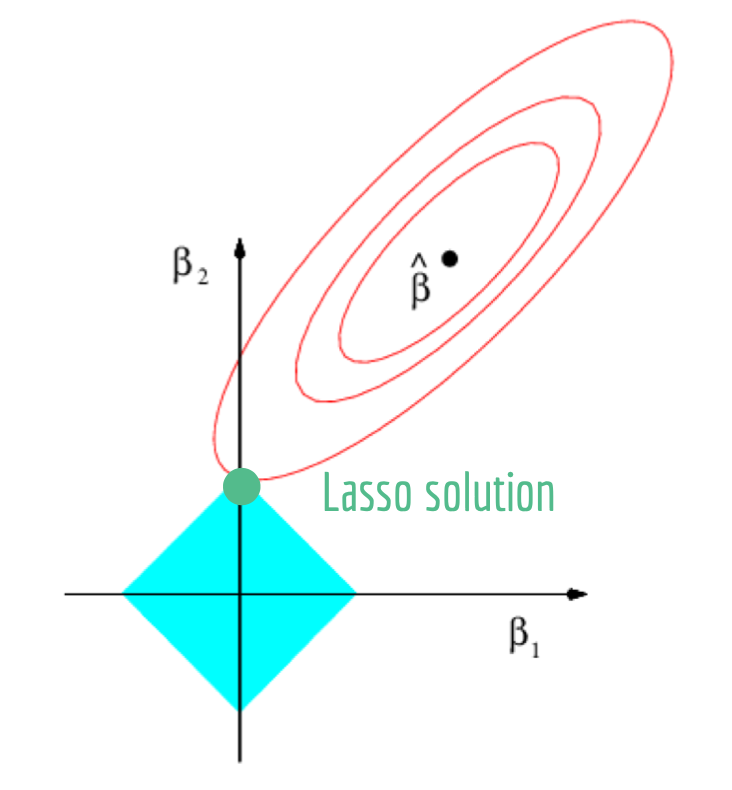
\includegraphics{lasso_vis.png}

\textbf{relationship between s and lambda???}

\hypertarget{selecting-the-tuning-parameter}{%
\subsubsection{Selecting the Tuning
Parameter}\label{selecting-the-tuning-parameter}}

\hypertarget{comparison-to-ridge-regression}{%
\subsubsection{Comparison to Ridge
Regression}\label{comparison-to-ridge-regression}}

Ridge regression is another technique that modifies the OLS framework by
constraining the values of the coefficients. Ridge regression is defined
as:
\[\text{argmin}_{\beta_j}\sum_{i=1}^n ( y_i +\beta_0 - \sum_{j=1}^p \beta_jx_{ij} )^2 + \color{red}{\lambda \sum_{j=1}^p (\beta_j)^2}\].
We can see that ridge regression is nearly identical to lasso; the only
difference is in the penalty term (shown above in red). Instead of
taking the absolute value of the coefficients, ridge regression squares
the coefficients. We can consider the constrained optimization
formulation of ridge regression, as we did for lasso: \[
\text{argmin}_{\beta_j}\sum_{i=1}^n ( y_i +\beta_0 - \sum_{j=1}^p \beta_jx_{ij} )^2  \text{; subject to }  \sum_{j=1}^p (\beta_j)^2 \le s.
\] With two predictors, the constraint region becomes a circle:
\(\beta_1^2 + \beta_2^2 \le s^2\). We can construct a very similar graph
to the one above:

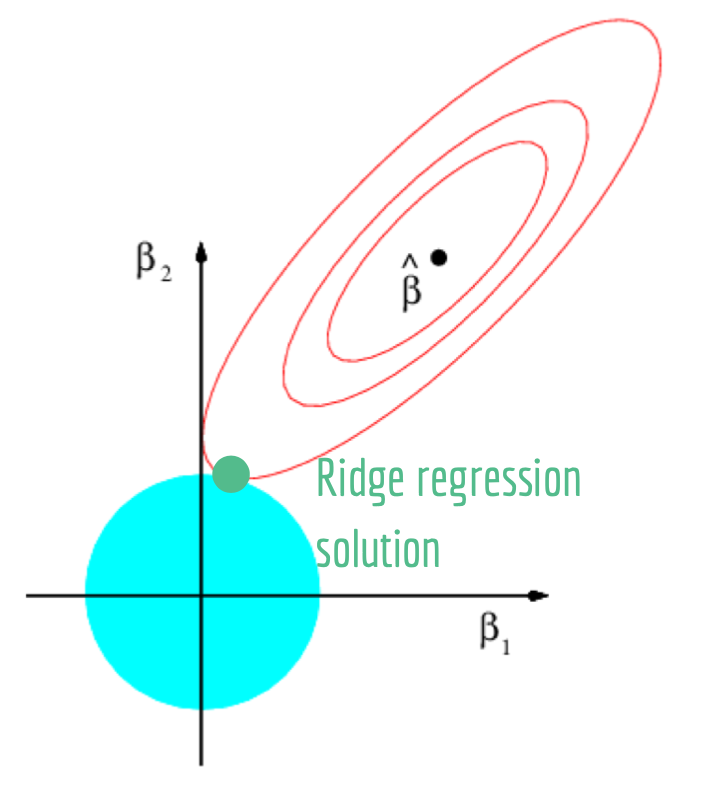
\includegraphics{ridge_vis.png} The only difference between lasso and
ridge regression are their constraint regions.

\hypertarget{benefits-of-lasso-and-ridge-regression}{%
\subsubsection{Benefits of Lasso and Ridge
Regression}\label{benefits-of-lasso-and-ridge-regression}}

\hypertarget{main-results}{%
\subsection{Main Results}\label{main-results}}

\hypertarget{deriving-ols-ridge-regression-and-lasso-estimators}{%
\subsubsection{Deriving OLS, Ridge Regression and Lasso
Estimators}\label{deriving-ols-ridge-regression-and-lasso-estimators}}

\hypertarget{ols}{%
\paragraph{OLS}\label{ols}}

As described above, the OLS problem can be written as
\(\text{argmin}_{\boldsymbol\beta} (\mathbf{y} - \mathbf{X}\boldsymbol\beta)^\top(\mathbf{y} - \mathbf{X}\boldsymbol\beta)\).

We can derive the OLS estimate for \(\boldsymbol\beta\): \$\$

\begin{aligned}

\text{argmin}_{\boldsymbol\beta} (\mathbf{y} - \mathbf{X}\boldsymbol\beta)^\top(\mathbf{y} - \mathbf{X}\boldsymbol\beta) \\ 

= \frac{\partial}{\partial \boldsymbol\beta} (\mathbf{y}^\top \mathbf{y} - \mathbf{y}^\top\mathbf{X}\boldsymbol\beta  - \boldsymbol\beta^T\mathbf{X}^Ty + \boldsymbol\beta^\top \mathbf{X}^\top \mathbf{X} \boldsymbol\beta) \\

= \frac{\partial}{\partial \boldsymbol\beta} (\mathbf{y}^\top \mathbf{y} - 2\mathbf{y}^\top\mathbf{X}\boldsymbol\beta + \boldsymbol\beta^\top \mathbf{X}^\top \mathbf{X} \boldsymbol\beta) \\

= -2\mathbf{X}^\top\mathbf{y} + 2 \mathbf{X}^\top \mathbf{X} \boldsymbol\beta \\

0 \stackrel{set}{=} -2\mathbf{X}^\top\mathbf{y} + 2 \mathbf{X}^\top \mathbf{X} \boldsymbol\beta \\

2 \mathbf{X}^\top \mathbf{X} \boldsymbol\beta = 2\mathbf{X}^\top\mathbf{y} \\ 

(\mathbf{X}^T\mathbf{X})^{-1}\mathbf{X}^\top \mathbf{X} \boldsymbol\beta = (\mathbf{X}^T\mathbf{X})^{-1} \mathbf{X}^\top\mathbf{y} \\ 

 \boldsymbol\beta = (\mathbf{X}^T\mathbf{X})^{-1} \mathbf{X}^\top\mathbf{y}

\end{aligned}

\$\$ \#\#\#\# Ridge Regression

In ridge regression, the formula we are trying to minimize is
\(\sum_{i=1}^n(y_i - \beta_0 - \sum_{j=1}^p\beta_j x_{ij})^2 + \lambda\sum_{j=1}^p \beta_j^2\).
We can write this in matrix notation as:
\((\mathbf{y} - \mathbf{X}\boldsymbol\beta)^\top(\mathbf{y} - \mathbf{X}\boldsymbol\beta) + \lambda \boldsymbol\beta^T\boldsymbol\beta\).
We can minimize this in much the same way as in OLS:

\$\$

\begin{aligned}

\text{argmin}_{\boldsymbol\beta} (\mathbf{y} - \mathbf{X}\boldsymbol\beta)^\top(\mathbf{y} - \mathbf{X}\boldsymbol\beta) + \lambda \boldsymbol\beta^T\boldsymbol\beta \\ 

= \frac{\partial}{\partial \boldsymbol\beta} (\mathbf{y}^\top \mathbf{y} - 2\mathbf{y}^\top\mathbf{X}\boldsymbol\beta + \boldsymbol\beta^\top \mathbf{X}^\top \mathbf{X} \boldsymbol\beta + \lambda \boldsymbol\beta^T\boldsymbol\beta) \\

= -2\mathbf{X}^\top\mathbf{y} + 2 \mathbf{X}^\top \mathbf{X} \boldsymbol\beta + 2\lambda\boldsymbol\beta \\

0 \stackrel{set}{=} -2\mathbf{X}^\top\mathbf{y} + 2 \mathbf{X}^\top \mathbf{X} \boldsymbol\beta + 2\lambda\boldsymbol\beta\\

\mathbf{X}^\top \mathbf{X} \boldsymbol\beta + \lambda\boldsymbol\beta = \mathbf{X}^\top\mathbf{y} \\ 

(\mathbf{X}^\top \mathbf{X} + \lambda\mathbf{I}) \boldsymbol\beta = \mathbf{X}^\top\mathbf{y} \\ 

(\mathbf{X}^\top \mathbf{X} + \lambda\mathbf{I}) (\mathbf{X}^\top \mathbf{X} + \lambda\mathbf{I}) ^{-1}\boldsymbol\beta = \mathbf{X}^\top\mathbf{y}(\mathbf{X}^\top \mathbf{X} + \lambda\mathbf{I}) ^{-1}\\ 

\boldsymbol\beta = \mathbf{X}^\top\mathbf{y}(\mathbf{X}^\top \mathbf{X} + \lambda\mathbf{I}) ^{-1}\\ 

\end{aligned}

\$\$

\hypertarget{considering-a-simple-case}{%
\paragraph{Considering a Simple Case}\label{considering-a-simple-case}}

We can consider a simple case: \(\mathbf{X}\) is a diagonal matrix with
1's on the diagonals and 0's on all the off diagonals, the number of
predictors equals the number of cases, and we force the intercept to go
through the origin. This case allows us simplify our OLS and ridge
regression estimators. For OLS, the solution is
\(\boldsymbol\beta = \mathbf{y}\) and for ridge regression the solution
becomes \(\boldsymbol\beta = \frac{\mathbf{y}}{1+\lambda}\). Applying
this simple case to find the estimators is helpful particularly for
Lasso. Unlike OLS and Ridge Regression, there is no closed form solution
for \(\boldsymbol\beta\) for Lasso. To derive any estimators for Lasso,
we must consider this simple case.

\hypertarget{lasso-estimators-in-a-simple-case}{%
\paragraph{Lasso Estimators in a Simple
Case}\label{lasso-estimators-in-a-simple-case}}

For lasso, we can not find a general closed form solution for
\(\boldsymbol\beta\), so we will derive the lasso estimates for
\(\boldsymbol\beta\) for the simple case described above. We will not
use matrix notation in order to easily apply the assumptions of our
simple case.

Remember that we can write the general form of lasso as:

\$\$

\begin{aligned}

\text{argmin}_{\beta}\sum_{i=1}^n(y_i - \beta_0 - \sum_{j=1}^p\beta_j x_{ij})^2 + \lambda\sum_{j=1}^p |\beta_j|

\end{aligned}

\$\$ If we apply our simplifying assumptions, we can write:

\$\$

\begin{aligned}

\text{argmin}_{\beta}\sum_{j=1}^p(y_i - \beta_1)^2 + \lambda|\beta_1| 

\end{aligned}

\$\$

With these assumptions, we can find a closed form solution for
\(\beta\):

\$\$

\begin{aligned}

\text{argmin}_{\beta}(y_i - \beta_1)^2 + \lambda|\beta_1| \\ 

= \frac{\partial}{\partial \beta} \left( (y_j - \beta_1)^2 + \lambda|\beta_1| \right) \\

= \frac{\partial}{\partial \beta} \left( y_j^2 - 2y_j\beta_1 + \beta_1^2 + \lambda|\beta_1| \right) \\

=  - 2y_j + 2\beta_1 + \lambda sign(\beta_1) \\

\end{aligned}

\$\$ To solve for \(\beta_1\), we must consider different regions: (1)
when \(\beta_1 < 0\), (2) when \(\beta_1 > 0\) and (3) when
\(\beta_1 = 0\).

\begin{enumerate}
\def\labelenumi{(\arabic{enumi})}
\tightlist
\item
  when \(\beta_1 < 0\) or when \(y_j < - \lambda/2\):
\end{enumerate}

\$\$ \textbackslash begin\{aligned\}

0 \stackrel{set}{=} - 2y\_j + 2\beta\_1 - \lambda \textbackslash{}

\beta\_1 = y\_j + \lambda/2 \textbackslash{}

\textbackslash{} \[
(2) when $\beta_1 > 0$ or when $y_j > \lambda/2$: 
\]

0 \stackrel{set}{=} - 2y\_j + 2\beta\_1 + \lambda \textbackslash{}

\beta\_1 = y\_j - \lambda/2 \textbackslash{}

\textbackslash{}

\[
(3) when $\beta_1 = 0$ ASK KELSEY
\]

\text{when } \beta\_1 = 0 \text{ or when }----: \textbackslash{}

0 \text{ when } \textbar y\_i\textbar{} \le \lambda/2

\$\$

\hypertarget{visualizing-the-simple-case-estimators}{%
\paragraph{Visualizing the Simple Case
Estimators}\label{visualizing-the-simple-case-estimators}}

\begin{Shaded}
\begin{Highlighting}[]
\FunctionTok{library}\NormalTok{(ggplot2)}
\NormalTok{lambda }\OtherTok{\textless{}{-}} \DecValTok{5}
\NormalTok{ols }\OtherTok{\textless{}{-}} \ControlFlowTok{function}\NormalTok{(x) x}
\NormalTok{ridge }\OtherTok{\textless{}{-}} \ControlFlowTok{function}\NormalTok{(x) x}\SpecialCharTok{/}\NormalTok{(}\DecValTok{1}\SpecialCharTok{+}\NormalTok{lambda)}
\NormalTok{lasso }\OtherTok{\textless{}{-}}\ControlFlowTok{function}\NormalTok{(x) }\FunctionTok{ifelse}\NormalTok{(x }\SpecialCharTok{\textgreater{}}\NormalTok{ lambda}\SpecialCharTok{/}\DecValTok{2}\NormalTok{, x}\SpecialCharTok{{-}}\NormalTok{lambda}\SpecialCharTok{/}\DecValTok{2}\NormalTok{,}
   \FunctionTok{ifelse}\NormalTok{(x }\SpecialCharTok{\textless{}} \SpecialCharTok{{-}}\NormalTok{lambda}\SpecialCharTok{/}\DecValTok{2}\NormalTok{, x}\SpecialCharTok{+}\NormalTok{lambda}\SpecialCharTok{/}\DecValTok{2}\NormalTok{, }
   \FunctionTok{ifelse}\NormalTok{( }\SpecialCharTok{{-}}\NormalTok{lambda}\SpecialCharTok{/}\DecValTok{2} \SpecialCharTok{\textless{}=}\NormalTok{ x }\SpecialCharTok{\&}\NormalTok{ x }\SpecialCharTok{\textless{}=}\NormalTok{ lambda}\SpecialCharTok{/}\DecValTok{2}\NormalTok{, }\DecValTok{0}\NormalTok{, }\DecValTok{0}\NormalTok{)))}


\FunctionTok{ggplot}\NormalTok{() }\SpecialCharTok{+}
  \FunctionTok{xlim}\NormalTok{(}\SpecialCharTok{{-}}\DecValTok{10}\NormalTok{, }\DecValTok{10}\NormalTok{)}\SpecialCharTok{+}
  \FunctionTok{geom\_function}\NormalTok{(}\AttributeTok{fun =}\NormalTok{ ols,}
                \FunctionTok{aes}\NormalTok{(}\AttributeTok{color =} \StringTok{\textquotesingle{}OLS\textquotesingle{}}\NormalTok{),}
                \AttributeTok{linetype =} \StringTok{"dashed"}\NormalTok{) }\SpecialCharTok{+}
  \FunctionTok{geom\_function}\NormalTok{ (}\AttributeTok{fun =}\NormalTok{ ridge,}
                 \FunctionTok{aes}\NormalTok{(}\AttributeTok{color =} \StringTok{\textquotesingle{}Ridge\textquotesingle{}}\NormalTok{),}
                 \AttributeTok{lwd =} \FloatTok{1.2}\NormalTok{)}\SpecialCharTok{+}
  \FunctionTok{geom\_function}\NormalTok{(}\AttributeTok{fun =}\NormalTok{ lasso,}
                \FunctionTok{aes}\NormalTok{(}\AttributeTok{color =} \StringTok{\textquotesingle{}Lasso\textquotesingle{}}\NormalTok{),}
                \AttributeTok{lwd =} \FloatTok{1.2}\NormalTok{) }\SpecialCharTok{+}
  \FunctionTok{theme\_bw}\NormalTok{()}\SpecialCharTok{+}
  \FunctionTok{theme}\NormalTok{(}\AttributeTok{panel.grid.minor.x =} \FunctionTok{element\_blank}\NormalTok{(),}
        \AttributeTok{panel.grid.minor.y =} \FunctionTok{element\_blank}\NormalTok{())}\SpecialCharTok{+}
  \FunctionTok{scale\_color\_manual}\NormalTok{(}\AttributeTok{name =} \StringTok{\textquotesingle{}Models\textquotesingle{}}\NormalTok{,}
                     \AttributeTok{breaks =} \FunctionTok{c}\NormalTok{(}\StringTok{\textquotesingle{}OLS\textquotesingle{}}\NormalTok{, }\StringTok{\textquotesingle{}Ridge\textquotesingle{}}\NormalTok{, }\StringTok{\textquotesingle{}Lasso\textquotesingle{}}\NormalTok{),}
                     \AttributeTok{values =} \FunctionTok{c}\NormalTok{(}\StringTok{\textquotesingle{}OLS\textquotesingle{}}\OtherTok{=}\StringTok{\textquotesingle{}gray54\textquotesingle{}}\NormalTok{, }\StringTok{\textquotesingle{}Ridge\textquotesingle{}}\OtherTok{=}\StringTok{\textquotesingle{}olivedrab3\textquotesingle{}}\NormalTok{, }\StringTok{\textquotesingle{}Lasso\textquotesingle{}}\OtherTok{=}\StringTok{\textquotesingle{}tan2\textquotesingle{}}\NormalTok{))}\SpecialCharTok{+}
  \FunctionTok{labs}\NormalTok{(}\AttributeTok{y =} \StringTok{"Coefficient Estimates"}\NormalTok{, }\AttributeTok{x =} \StringTok{"yj"}\NormalTok{)}
\end{Highlighting}
\end{Shaded}

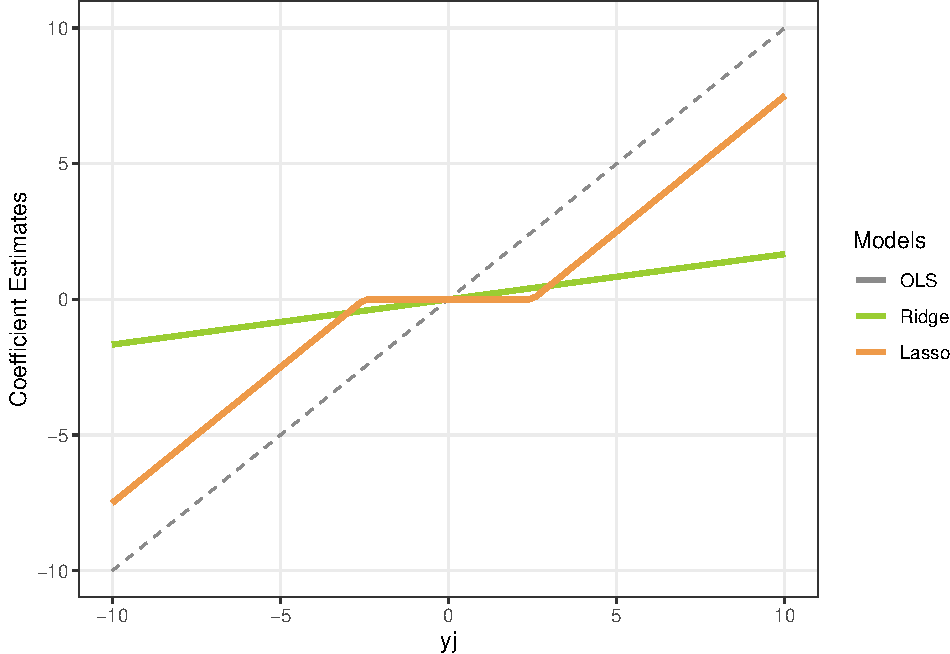
\includegraphics{Final-Project_files/figure-latex/unnamed-chunk-1-1.pdf}
DESCRIPTION OF WHAT THIS TELLS US

\hypertarget{simulation}{%
\subsubsection{Simulation}\label{simulation}}

\end{document}
